\chapter[Elements of Nuclear Physics]{Elements of Nuclear Physics}\label{chap3}

\Authorline{A. P. Balachandran\footnote{Email: \url{vdevanathan@hotmail.com}}}

\begin{center}
The Academy of Sciences, Chennai\\
Department of Nuclear Physics\\
University of Madras, Guindy Campus\\
Chennai - 600 025
\end{center}

\section*{Abstract}

\begin{quote}
The study of Nuclear Physics can be broadly classified into two parts; the static part and the dynamic part. The static part consists of the study of nuclear energy levels, their binding energies, the magnetic dipole moments and the electric quadrupole moments. The dynamic part deals with the transition of nuclei from one energy level to another due to interactions with external agencies including elementary particles. The former involves the evaluation of matrix elements with spherical tensor operators and the latter the calculation of transition probability from one nuclear state to another. This article briefly outlines how the transition probability can be calculated and how the method can be applied to the study of photoproduction of pions from nuclei. This was an emerging field, about sixty years ago, and this article presents some initial attempts made by G. Ramachandram and I to study this problem.
\end{quote}

\section{Introduction}\label{chap3-sec1}
 
 It was with Professor G. Ramachandran that I started to lern the elements of Nuclear Physics in he late Nineteen fifties when we commenced our research career \cite{key1,key2,key3,key4,key5,key6,key7,key8} under the guidance of Prof. Alladi Ramakrishnan, in the University of Madras. Earlier, Prof. Alladi had done remarkable work in the field of Stochastic Processes using the concept of Product Densities, known now as Ramakrishnan Product Densities. In the year 1958, he spent a year at the Institute for Advanced Studies at Princeton which had an exhilarating influence on him and his interest shifted from Stochastic Processes to Elementary Particles and Nuclear Physics. It had also brought about a great change in his vision and motivated him to create such a centre in India. On his return to India, he started one-year M.Sc. Course in Theoretical Physics which attracted a large number of brilliant students to join the course. Soon, he was promoted as Professor and posted to the newly started extension centre at Madurai but permitted to run the M.Sc. Program, already started, in Madras. It was a nebulous situation. Since Prof. Alladi had a palatial ancestral home - Ekamra Nivas, he conducted most of the classes in the spacious hall on the first floor of his house. Since Elementary particles and Nuclear Physics were new areas of study, everyone was encouraged to give lectures on different topics. The learning process may truly be called a boot-strap mechanism.

The informal group was given the name “Theoretical Physics Seminar” and we started inviting the visiting scientists from abroad to give talks at the Seminar. Visit to Mahabalipuram and dinner at New Woodlands were the usual way of extending the hospitality to the visiting scientists. A.M. Lane, Abdus Salam, Donald Glaser, S. Chandrasekhar were some of the distinguished scientists who gave talks at the Seminar. A few of them stayed as in-house guests of Prof. Alladi. They are scientists of high calibre. Donald Glaser already received the Nobel Prize for his invention of Bubble Chamber and Abdus Salam and S. Chandrasekhar received the Nobel Prizes subsequently. Abdus Salam was responsible for setting up the International Centre for Theoretical Physics at Trieste, which offered the opportunity for young scientists from developing countries to participate in its research activities as visiting scientists. Photographs of the Theoretical Physics Seminar Group taken with Abdus Salam, Donald Glaser and S. Chandrasekhar are attached herewith.
\eject

\begin{figure}[H]
\centering{
\includegraphics[scale=.75]{figures/chap3-fig1.eps}\\
Sitting: Dr. S.K. Srinivasan, Dr. Abdus Salam, Dr. A. Ramakrishnan, Mrs. Ramakrishnan, R. Thunga, T. K. Radha\\
Standing: xxxxxxxxxxx V. Devanathan, G. Ramachandran}
\end{figure}

\begin{figure}[H]
\centering{
\includegraphics[scale=.75]{figures/chap3-fig2.eps}\\
Front Row: R. Thunga, T. K. Radha, Dr. Donald Glaser (N.L.), Dr. A. Ramakrishnan, S. Indhumathi, G. Bhamathi\\
Second Row: A.P. Balachandran, K. Ananthanarayanan, K. Venkatesan, x, M.Deshpande, K. Raman, V. Devanathan, G. Ramachandran, Nambi Iyengar}
\end{figure}

\begin{figure}[H]
\centering{
\includegraphics[scale=.75]{figures/chap3-fig3.eps}\\
Front Row: S. Indhumathi, G. Bhamathi, Mrs. Ramakrishnan, Dr. A. Ramakrishnan, Dr. S. Chandrasekhar, T. K. Radha, R. Thunga;\\
Second Row: K. Raman, V. Devanathan, Dr. S. K. Srinivasan, K. Venkatesan, A. P. Balachandran, G. Ramachandran, x, Nambi Iyengar}
\end{figure}

It was a fortunate coincidence that both Niels Bohr and Abdus Salam visited Madras in January 1960, after attending the Indian Science Congress held at Bombay and the Theoretical Physics Seminar hosted a dinner in honour of both in New Woodlands. Niels Bohr was very much impressed by the efforts of Alladi in gathering a small enthusiastic group of young theoretical physicists and communicated the same to the then Prime Minister of India, Jawaharlal Nehru, which ultimately resulted in the establishment of the Institute of Mathematical Sciences at Madras 	on January 3, 1962 on the pattern of Institute for Advanced Studies at Princeton \cite{key9}.

At the Theoretical Physics Seminar, which was the forerunner of Institute of Mathematical Sciences, G. Ramachandran and I gave several lectures on different topics in Nuclear Physics. Prof. Manoj Banerji from Calcutta University was invited by the Seminar and he gave a series of lectures on Angular Momentum. G. Ramachandran and I found those lectures very useful since the study of Nuclear physics involves a lot of angular momentum algebra. The investigation of static properties of nuclei such as magnetic dipole moment, electric quadrupole moment and the various energy levels of nuclei involve the calculation of matrix elements between nuclear states using the spherical tensor operators. The study of the dynamical properties of nuclei due to nuclear transition from one state to another as a result of interaction with external field is more involved since it requires the calculation of transition probability of nucleus from one state to another besides the evaluation of matrix elements. If the magnetic sub-states of the initial and final nuclei are not observed, we need to sum over the final magnetic sub-states and average over the initial magnetic sub-states. When we started our research, the study of elementary particle reactions with nuclei was an emerging field and it involved a knowledge of both elementary particle interactions and nuclear structure. Since angular momentum is a conserved quantity in any reaction, a sound knowledge of angular momentum algebra is a pre-requisite for such a study. This has motivated G. Ramachandran to publish the Matscience Report on Angular Momentum \cite{key10} and V. Devanathan, at a later date, to write Text Books, one on Angular Momentum \cite{key11} and another on Nuclear Physics \cite{key12}.

In the year 1957, Chew et al (hereafter referred to as CGLN) \cite{key13} has obtained a general amplitude for photoproduction of pions from nucleons using dispersion relations. Around the same time, Hughes and March \cite{key14} attempted to study experimentally the nuclear transitions to individual final nuclear states by observing the radioactivity of the final nuclear state. He studied the reaction ${}^{11} B(\gamma, \pi^-)^{11} C$. This was followed by other activity measurements by Dyal and Hummel \cite{key15} on ${}^{11} B$, by March and Walker \cite{key16} on ${}^{60} N i$, by Meyer et al \cite{key17} on ${}^{16} O$ and ${}^{27} Al$ and by Nydall and Forkman \cite{key18} on ${}^{11} B$, ${}^{27} Al$ and ${}^{51} V$.

Since the elementary amplitude for photoproduction of pion from nucleon was known and the experimental investigations on nuclei were already initiated, Ramachandran and I \cite{key4, key5} started to formulate a theory for photo-pion production from nuclei using impulse approximation and plane waves for the incident photon and the emitted pion.

The theoretical study of photoproduction of pions from nuclei depends on four essential factors:
\begin{enumerate}
\item The elementary photopion production amplitude for the nucleons
\item The construction of the nuclear transition amplitude from the free nucleon amplitude
\item The final state interaction of the outgoing pion with the residual nucleus
\item The nuclear structure
\end{enumerate}

One can check the validity of the elementary photopion production amplitude by comparing the calculated cross section with the experimentally observed cross section for the elementary process on free nucleons. This only checks the on-shell behaviour of the amplitude. In the nuclear process, the off-shell behaviour also counts. Besides, multiple scattering effects should also be considered. The plane wave approximation for the incident photon may be valid but definitely not for the pion. The calculated cross section with the plane wave approximation for the emitted pion was much larger than the experimental cross section and a phenomenological surface production model \cite{key19} was invoked to obtain the fit with experiment. Later on, The distortion effects on the emitted pion \cite{key20,key21} was properly taken into account by solving the Klein-Gordon equation with a suitable optical potential for the radial wave function. It was found that the nuclear structure also plays a vital part in the reaction.

Although our initial effort is to obtain an analytical expression for the photopion cross section from nuclei using simplifying assumptions, later we have found that the distortion effects on the pion and nuclear structure play a dominant role. A comprehensive review \cite{key22} on Photo-pions from nuclei is available. 

In this article, we do not follow the chronological order in the presentation but follow the logical sequence by discussing the coupling rule for spherical tensor operators, the evaluation of nuclear matrix elements and nuclear transition probability under the influence of spherical tensor operators \cite{key12}. The photo-pion production from nuclei is presented here for illustrative purpose only.

Both the static and dynamic properties of nuclei are studied by calculating nuclear matrix elements using spherical tensor operators. The coupling rules for spherical tensor operators are presented in Sec. 2 as a prelude to the study of transition probability of nucleus from one state to another which is outlined in Sec. 3. In Sec. 4, we study the elementary photopion production reaction on nucleons. The study is extended to photopion production from nuclei in Sec. 5.1 using impulse approximation for the reaction process and plane waves for the incident photon and the emitted pion. The plane wave approximation for the incident photon is justifiable but not for the outgoing pion. How to include the distortion effects on the emitted pion is discussed in Sec. 5.2.

\section{Coupling rules for Spherical Tensor Operators} \label{chap3-sec2}

The spherical harmaonics $Y^m_l(\theta, \phi)= Y_l^m (\hat{\mathbf{r}})$ can be considered as spherical tensor operators and they obey the coupling rule
\begin{equation}
Y_{l_1}^{m_1} (\hat{\mathbf{r}}) Y_{l_2}^{m_2} (\hat{\mathbf{r}}) = \sum_L 
	\begin{bmatrix}
		l_1 & l_2 & L\\
		m_1 &m_2  & m_L
	\end{bmatrix}
(Y_{l_1} (\hat{\mathbf{r}}) \times Y_{l_2} (\hat{\mathbf{r}}))^{m_L}_{L}, \label{chap3-eq1}
\end{equation}
where
\begin{equation}
(Y_{l_1}  (\hat{\mathbf{r}})  \times Y_{l_2} (\hat{\mathbf{r}}) )^{m_L}_{L} = \frac{[l_1][l_2]}{\sqrt{4\pi}[L]}
\begin{bmatrix}
l_1 & l_2 & L\\
0 & 0 & 0
\end{bmatrix}
Y_{L}^{m_L} (\hat{\mathbf{r}}). \label{chap3-eq2} 
\end{equation}
For brevity, the symbol $[l]$ is used to denote $[l] = 2l + 1$. The wide square bracket represents the Clebsch-Gordan (C.G.) coefficient. For the notations and symbols, kindly refer to Devanathan \cite{key11,key12}. \eqref{chap3-eq2} is applicable only to spherical harmonics but the definition \eqref{chap3-eq1} can be extended to any spherical tensor operators.

Let $A_{l_1}^{m_1}$ and $B_{l_2}^{m_2}$ be the components of any two spherical tensor operators of ranks $l_1$ and $l_2$. Then we can construct a tensor product $(A_{l_1} \times B_{l_2})^M_L$ using C.G. coefficients.
\begin{equation}
(A_{l_1} \times B_{l_2})^M_L \sum_{m_1 ~m_2} 
\begin{bmatrix}
  l_1 & l_2 & L\\
  m_1 & m_2 & M
\end{bmatrix}
A_{l_1}^{m_1} B_{l_2}^{m_2}.  \label{chap3-eq3}
\end{equation}
In the special case In the special case of $L = 0$, we can write $l_1 = l_2 = l$ and $m_1 = −m_2 = m$ and the
tensor product can be expressed as a scalar product with a factor as shown in \eqref{chap3-eq4}.
\begin{align}
  (A_l \times B_l)^0_0 & = \sum_{m}
  \begin{bmatrix}  l & l & 0\\    m & -m & 0  \end{bmatrix}  A_l^m B_l^{-m}\notag\\
  & = \sum_m (-1)^{l-m} \frac{1}{[l]}
  \begin{bmatrix}    l & 0 & l\\    m & 0 & m  \end{bmatrix}  A_l^m B_l^{-m}\notag\\
  & = \frac{(-1)^l}{[l]} a_l \cdot B_l, \label{chap3-eq4}
\end{align}
using the notation $[l] = \bar{2l + 1}$. One can write the inverse relation of \eqref{chap3-eq3}. Given any two spherical tensor operators $A_{l_1}^{m_1}$, $A_{l_2}^{m_2}$, they can be expressed as a linear sum of tensor products $(A_{l_1} \times B_{l_2})^M_L$, with $|l_1 − l_2 | \leq L \leq l_1 + l_2$ 
\begin{equation}
A_{l_1}^{m_1} A_{l_2}^{m_2} = \sum_{L} 
\begin{bmatrix}
l_1 & l_2 &L\\
m_1 & m_2 & M
\end{bmatrix} (A_{l_1} \times B_{l_2})^M_L. \label{chap3-eq5}
\end{equation}

If there are three tensor operators $A_{l_1}$, $B_{l_2}$, $C_{l_3}$ , then it is possible to form a tensor product of them in more than one way: \eqref{chap3-eq1} by coupling $A_{l_1}$, $B_{l_2}$ and then coupling the resultant with $C_{l_3}$ or \eqref{chap3-eq2} by coupling $B_{l_2}$, $C_{l_3}$ first and then coupling $A_{l_1}$ with the resultant, as indicated below:
\begin{equation}
\left[ (A_{l_1} \times B_{l_2})_{l_{12}} \times C_{l_3}\right]^M_L;  \qquad \left[ A_{l_1} \times (B_{l_2} \times C_{l_3})_{l_{23}}\right]^M_L. \label{chap3-eq6}
\end{equation}
One can go from on coupling scheme to another by a unitary transformation,
\begin{align}
\left[ (A_{l_1} \times B_{l_2})_{l_{12}} \times C_{l_3}\right]^M_L  & = \sum_{l_{23}} U (l_1, l_2 L l_3, l_{12} l_{23}) 
\left[A_{l_1} \times (B_{l_2} \times C_{l_3})_{l_{23}} \right]^M_L. \label{chap3-eq7}\\ 
\left[ A_{l_1} \times (B_{l_2} \times C_{l_3})_{l_{23}}\right]^M_L & = \sum_{l_{12}} U (l_1, l_2 L l_3, l_{12} l_{23}) 
\left[(A_{l_1} \times B_{l_2})_{l_{12}} \times C_{l_3}) \right]^M_L. \label{chap3-eq8} 
\end{align}
The unitary transformation coefficients $U (l_1 l_2 L l_3, l_{12} l_{23})$ defined in Eqs. \eqref{chap3-eq7} and \eqref{chap3-eq8} are exactly the recoupling coefficients that occur in the addition of three angular momenta \cite{key11,key12}. The recoupling coefficient $U (l_1 l_2 Ll_3 , l_{12} l_{23})$ can be expressed in terms of Racah coefficient $W (l_1 l_2 Ll_3 , l_{12} l_{23})$ 
\begin{equation}
U (l_1 l_2 Ll_3 , l_{12} l_{23}) = [l_{12}][l_{23}] W (l_{1} l_2 Ll_3 , l_{12} l_{23}). \label{chap3-eq9}
\end{equation}
If there are four spherical tensor operators $A_{l_1}, B_{l_2}, C_{l_3}, D_{l_4}$ of ranks $l_1, l_2, l_3, l_4$ respectively, then also one can construct tensor product of them in more than one way: \eqref{chap3-eq1} by coupling $A_{l_1}, B_{l_2}$ and $C_{l_3}, D_{l_4}$ separately to form tensors of rank $l_{12}$ and $l_{34}$ and then coupling these resultant tensors to form the product tensor of rank $L$ or \eqref{chap3-eq2} by coupling $A_{l_1}, C_{l_3}$ and $B_{l_2}, D_{l_4}$ initially to obtain the tensor products of rank $l_{13}$ and $l_{24}$ and then coupling these resultant tensors to obtain the product tensor of rank $L$. These two different ways of coupling correspond to two different representations and one can go from one representation to another representation by a unitary transformation, using the re-coupling coefficient. This is similar to the re-coupling coefficient that occur in the addition of four angular momenta \cite{key11,key12}.

\begin{align}
& [(A_{l_1} \times B_{l_2})_{l_{12}} \times (C_{l_3} \times D_{l_4})_{l_{34}}]^M_L \notag \\
& \qquad = \sum_{l_{13} l_{24}}
	\begin{bmatrix}l_1 & l_2 & l_{12}\\l_3 & l_4 & l_{34}\\l_{13} & l_{24} & L\end{bmatrix}
	\times [(A_{l_1} \times C_{l_3})_{l_{13}} \times (B_{l_2} \times D_{l_4})_{l_{24}}]^M_L. \label{chap3-eq10}\\
& [(A_{l_1} \times C_{l_3})_{l_{13}} \times (B_{l_2} \times D_{l_4})_{l_{24}}]^M_L  \notag \\
& \qquad = \sum_{l_{12} l_{34}}
	\begin{bmatrix}l_1 & l_2 & l_{12}\\l_3 & l_4 & l_{34}\\l_{13} & l_{24} & L\end{bmatrix} 
	\times [(A_{l_1} \times B_{l_2})_{l_{12}} \times (C_{l_3} \times D_{l_4})_{l_{34}}]^M_L. \label{chap3-eq11}
\end{align}
The recoupling coefficient (denoted by wide square brackets) that occurs in the coupling of four spherical tensors can be expressed in terms of Wigner's 9-j symbol (denoted by wide curly brackets).
\begin{equation}
	\begin{bmatrix}l_1 & l_2 & l_{12}\\l_3 & l_4 & l_{34}\\l_{13} & l_{24} & L\end{bmatrix} 
	= [l_{12}] [l_{34}] [l_{13}] [l_{24}] 
	\left\{\begin{matrix}l_1 & l_2 & l_{12}\\l_3 & l_4 & l_{34}\\l_{13} & l_{24} & L\end{matrix} \right\} \label{chap3-eq12}
\end{equation}

\subsection{Nuclear Matrix clements of spherical tensor operators}\label{chap3-sec2.1}

Let us now consider the evaluation of the following two-body matrix elements of spherical tensor operators:
\begin{align}
(1) ~ Q_1 & = \langle j_1' j_2' j' m' |A_k^\mu (1)| j_1 j_2 j m \rangle \label{chap3-eq13}\\
(2) ~ Q_2 & = \langle j_1' j_2' j' m' |B_k^\mu (2)| j_1 j_2 j m \rangle \label{chap3-eq14}\\
(3) ~ Q_3 & = \langle j_1' j_2' j' m' |(A_{k_1} (1) \times B_{k_2} (2))_k^\mu  | j_1 j_2 j m \rangle \label{chap3-eq15}
\end{align}

\medskip
\noindent \textbf{\large Evaluation by using recoupling coefficients}
\medskip

\noindent First let us evaluate the matrix element $Q_2$. Using the Wigner-Eckart theorem,
\begin{equation}
A_2 \begin{bmatrix}j & k & j'\\m & \mu & m'\end{bmatrix}
\langle j_1' j_2' j' || B_k (2) || j_1 j_2 j \rangle \delta_{j_1 j_1'}. \label{chap3-eq16}
\end{equation}
Since the operator acts on particle 2 only, the angular momentum of particle 1 is unaffected. In addition, the two-body reduced matrix element can be expressed in terms of one-body matrix element using the concept of recoupling coefficient $U$. The two-body matrix element corresponds to the coupling scheme of three angular momenta\footnote{The bold-face letters $\mathbf{J}_1, \mathbf{J}_2, \mathbf{J}, \cdots$ are used to denote the angular momentum vectors whereas the corresponging lower case letters $j_1, j_2, j, \cdots$ denote the angular momentum quantum numbers.}
$$
\mathbf{J}_1 + \mathbf{J}_2 = \mathbf{J}, \qquad \mathbf{J}+ \mathbf{K}= \mathbf{J}',
$$
whereas the one-body marix element corresponds to the coupling scheme
$$
\mathbf{J}_2 + \mathbf{K} = \mathbf{J}_2', \qquad \mathbf{J}_1+ \mathbf{J}_2'= \mathbf{J}'.
$$
One can go from one coupling scheme to the other by using the unitary transformation coefficient $U(j_1 j_2 j' k, j j_2')$.
\begin{equation}
\langle j_1 j_2' j' || B_k (2) || j_1 j_2 j \rangle = U (j_1 j_2 j' k, j j_2') \langle j_2' || B_k (2) || j_2 \label{chap3-eq17}
\end{equation}
Substituting \eqref{chap3-eq17} into Eq. \eqref{chap3-eq16}, we obtain
\begin{equation}
Q_2 = \begin{bmatrix}j & k & j'\\m & \mu & m'\end{bmatrix}
U (j_1 j_2 j' k, j j_2') \langle j_2' || B_k (2) || j_2 \label{chap3-eq18}
\end{equation}

Having evaluated $Q_2$, we shall now evaluate $Q_1$. In $Q_1$, the transition operator $A_k^\mu$ \eqref{chap3-eq1} corresponds to particle 1. Switching particles 1 and 2 in the ket and bra vectors of two-particle system introduces a phase factor\footnote{The phase factor $(-1)^{j_1 +j_2-j}$ is either $+1$ or $-1$. This means $j_1 + j_2-j$ is either and even or odd integer.}  as shown below:
\begin{align}
| j_1 j_2 j m 
& = \sum_{m_1m_2} \begin{bmatrix}j_1 & j_2 & j\\m_1 & m_2 & m\end{bmatrix} |j_1 m_1 \rangle| j_2 m_2\rangle \notag \\
& = (-1)^{j_1 j_2-j} \sum_{m_1 m_2} 
	\begin{bmatrix}j_2 & j_1 & j\\m_2 & m_1 & m \end{bmatrix} |j_1 m_1 \rangle | j_2 m_2 \rangle \notag \\
& = (-1)^{j_1 + j_2-j} | j_2 j_1 j m \rangle .\label{chap3-eq19}
\end{align}
Similarly,
\begin{equation}
|j_1' j_2 j' m' \rangle = (-1)^{j_1' + j_2 - j'} | j_2 j_1' j' m' \rangle . \label{chap3-eq20}
\end{equation}
Hence\footnote{The product of two phase factors $(-1)^{n_1} (-1)^{n_2}$ can be written either as $(-1)^{n_1 + n_2}$ or as $(-1)^{n_1-n_2}$, since $n_1$ and $n_2$ are integers (either odd or even).}
\begin{align}
Q_1 & = (-1)^{j_1 + j_2 -j} (-1)^{j_1' + j_2 -j' }
	\begin{bmatrix}j_1 & j_2 & j\\m_1 & m_2 & m\end{bmatrix} | j_1 m_1 \rangle | j_2 m_2 \rangle \notag \\
& = (-1)^{j_1 j_2-j} \sum_{m_1 m_2}
\begin{bmatrix}j_2 & j_1 & j\\m_2 & m_1 & m\end{bmatrix} | j_1 m_1 \rangle | j_2 m_2 \rangle \notag \\
& = (-1)^{j_1+j_2-j} | j_2 j_1 jm \rangle. \label{chap3-eq21}
\end{align}
The last step is obtained using Eq. \eqref{chap3-eq17}. Only the subscripts 1 and 2 are interchanged. 

We shall now evaluate $Q_3$. Applying the Wigner-Eckart theorem,
%%% Start page no 10

\begin{thebibliography}{99}
\bibitem{key1} V. Devanathan and G. Ramachandran, \textit{A note on photomesons from deuterons}, Nuclear Physics \textbf{23}, 312 (1961).
\bibitem{key2} A. Ramakrishnan, G. Ramachandran and V. Devanathan, \textit{Elastic Photoproduction of neutral pions from deuterons}, Nuclear Physics \textbf{24}, 163 (1961).
\bibitem{key3} A. Ramakrishnan, G. Ramachandran and V. Devanathan, \textit{A time dependent approach to rearrangement collisions}, Nuovo cimento \textbf{21}, 145 (1961).
\bibitem{key4} V. Devanathan and G. Ramachandran, \textit{Photoproduction of charged pions from nuclei-I}, Nuclear Physics \textbf{38},654 (1962).
\bibitem{key5} V. Devanathan and G. Ramachandran, \textit{Photoproduction of charged pions from nuclei-II}, Nuclear Physics \textbf{42}, 254 (1963).
\bibitem{key6} G. Ramachandran and V. Devanathan, \textit{Nuclear Polarization following Photoproduction of pions from nuclei-I}, Nuclear Physics \textbf{48}, 369 (1963).
\bibitem{key7} G. Ramachandran and V. Devanathan, \textit{Nuclear polarization following Photoproduction of pions from nuclei-II}, Nuclear Physics \textbf{50}, 593 (1964).
\bibitem{key8} V. Devanathan, R. Parthasarathy and G. Ramachandran, \textit{Polarization of the emitted Neutron in Muon Capture}, Ann. Phys. (N.Y) \textbf{72}, 428 (1972).
\bibitem{key9} Krishnaswami Alladi (Ed.), \textit{Alladi Diary, Memoirs of Alladi Ramakrishnan}, World Scientific (2019).
\bibitem{key10} G. Ramachandran, \textit{Matscience Report on Angular Momentum}, The Institute of Mathematical Sciences, Madras (1962)
\bibitem{key11} V. Devanathan, \textit{Angular Momentum Techniques in Quantum Mechanics}, Kluwer Academic Publishers, The Netherlands (1999)
\bibitem{key12} V. Devanathan, \textit{Nuclear Physics, 2nd Ed.,} Narosa Publishing House, New Delhi (2011).
\bibitem{key13} G. F. Chew, M. L. Goldberger, F. E. Low and Y. Nambu, Phys. Rev. \textbf{106}, 1345 (1957).
\bibitem{key14} I. S. Hughes and P. V. March, Proc. Phys. Soc. (London), \textbf{72}, 259 (1958)
\bibitem{key15} P. Dyal and J. P. Hummel, Phys. Rev. \textbf{127}, 2217 (1962)
\bibitem{key16} P. V. March and J. G. Walker, Proc. Phys. Soc. (London), \textbf{77}m 293 (1960)
\bibitem{key17} R. A. Meyer, W. B. Walters and J. P. Hummel, Phys. Rev. \textbf{B138}, 1421 (1965)
\bibitem{key18} G. Nydahl and B. Forkman, Nucl. Phys. \textbf{B7}, 97(1968)
\bibitem{key19} V. Devanathan, M. Rho, K. Srinivasa Rao and S.C.K. Nair, Nucl. Phys. \textbf{B2}, 329 (1967)
\bibitem{key20} V. Devanathan, in "Symposia in Theoretical Physics and Mathematics” (A. Ramakrishnan, Ed.), Vol. 10, p. 123, Plenum Press, New York (1970)
\bibitem{key21} V. Devanathan, V. Girija and G.N. Sivarama Prasad, Canadian Journal of Physics, \textbf{58}, 1151 (1980)
\bibitem{key22} A. Nagl, V. Devanathan, H. Überall, \textit{Nuclear Pion Photoproduction}, Springer-Verlag (1991)
\bibitem{key23} V. Devanathan, \textit{Quantum Mechanics, 2nd Ed.,} Narosa Publishing House, New Delhi (2011)
\bibitem{key24} V. Devanathan, \textit{The concept of phase-space in Quantum Mechanics}, Journal of Chennai Academy of Sciences, \textbf{2}, 26-42 (2020)
\end{thebibliography}
